
% Define document title and author
	\title{Tarea 1:\\VGG, ResNET and Squeeze \& Excitation}
	\author{Martin N. Valderrama\\ CC7221 - Reconocimiento de Imágenes con Deep Learning, Otoño 2020\\}
% 	\markboth{}{}
	\maketitle

% Write abstract here
\begin{abstract}

    En esta tarea se construyen y evalúan distintos modelos de redes convolucionales, sobre el framework Keras, con la finalidad de aprender la utilización del mismo, además de aprender a manipular redes neuronales. Se evalúa sobre un set de imágenes que corresponden a sketches o dibujos de 250 clases de objetos. Se obtienen resultados de bajo desempeño para un problema de clasificación de estas proporciones, cercano a 0.55 de \textit{accuracy} para cada modelo.
    
\end{abstract}

\section{Introducción}

    Las redes neuronales cada vez cobran mayor importancia en distintos ámbitos de la academia y la industria, se utilizan en áreas de reconocimiento de imágenes en su mayoría, pero también son utilizadas para la estimación de estadísticos en el ámbito de teoría de la información. En este informe se abordará la primera aplicación, donde se utilizarán tres arquitecturas distintas para clasificación de imágenes. Se verá la capacidad de cada una de las redes de generalizar y de ser capaces de distinguir entre las clases del problema.
    
    La base de datos a utilizar para el problema de clasificación es una compuesta por imágenes de sketches de distintos objetos. Algunos ejemplos son mostrados en la imagen (), cada una de ellas está compuesta por $256 \ \times \ 256$ pixeles, y la componen un total de 250 clases diferentes.
    
    La metodología a utilizar consiste en construir las redes sobre la plataforma de desarrollo Gooogle colaboratory, la cual consiste en clusters en línea que prestan la capacidad de procesamiento de gpus de alto rendimiento. Con ello el tiempo de entrenamiento de la red neuronal en cuestión disminuye radicalmente. Sobre esta plataforma se construyen las redes y luego se entrenan con una partición de la base de datos, mientras con el otro trozo se va evaluando el desempeño del modelo para lograr obtener el mejor rendimiento y capacidad de generalización de la red.
    
    Con esta tarea se busca entrenar la implementación de distintas arquitecturas y así dar las herramientas al estudiante de crear sus propias redes, realizar modificaciones y obtener los mejores modelos para la tarea asignada. Con ello, además se busca aplicar modelos de estado del arte en clasificación, intentando sacar el mayor provecho a la arquitectura propuesta.
    
    Si bien el buen rendimiento es deseado, el enfoque de la tarea es poder y lograr implementar las redes neuronales, ver las fases de entrenamiento y poder ajustar los parámetros para obtener un rendimiento aceptable.
    
    En este informe se verá el manejo del dataset para que las redes puedan entrenar, se revisa la implementación de las redes y su posterior entrenamiento. Finalmente, se evalúa su desempeño con los clásicos gráficos de función de pérdida y accuracy, donde se dan comentarios del comportamiento presentado. Se termina con reflexión del aprendizaje obtenido.


\section{Dataset}

    El dataset utilizado para realizar estos experimentos, es el realizado por (REFERENCIA A DATASET!) donde consiguen construir una base de datos de 20.000 imágenes con 250 clases diferentes de objetos dibujados a mano por humanos. El dataset está uniformemente distribuido, y por parte del cuerpo docente se separa en entrenamiento y test, donde el de entrenamiento es entregado completamente a la red para ajustar los pesos, mientras que se mira el rendimiento sobre el conjunto de test para evaluar el mismo entrenamiento, y de esta forma escoger el mejor modelo.
    
    \begin{figure}[t]
        \centering
        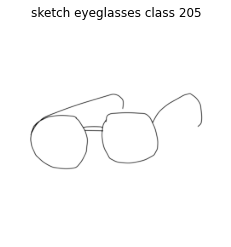
\includegraphics[width=0.2\textwidth]{img/glasses.png}
        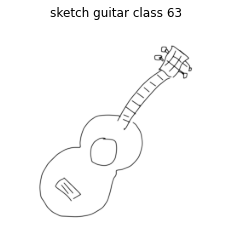
\includegraphics[width=0.2\textwidth]{img/guitar.png}
        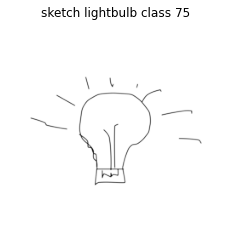
\includegraphics[width=0.2\textwidth]{img/bulb.png}
        \caption{Algunas imágenes que componen el dataset de (REFERENCIA DE PAPER DE DATOS). El tamaño de las imágenes es de $256 \times 256$ y en escala de grises.}
        \label{fig:dataset}
    \end{figure}
    
    El dataset consiste en dibujos a mano de 250 clases de objetos y animales de la vida cotidiana. Algunos ejemplos se pueden apreciar en la figura \ref{fig:dataset}. Se realiza una separación de los datos por parte del cuerpo docente, entre datos de entrenamiento 16000 imágenes y 4000 imágenes restantes para test o validación.
    
\section{Arquitecturas}
    
    La construcción de las redes es la propuesta por el enunciado de la tarea, con menores modificaciones ya que algunas sugerencias fueron hechas al momento de entrenar. Las modificaciones se vieron reflejadas en las últimas capas de la red, y tienen que ver con mejorar el desempeño de la red y mejorar la regularización y los resultados en el conjunto de validación.
    
    
    \subsection{VGG}
        
        Es una arquitectura de redes que se basa en el uso de filtros pequeños por cada capa convolucional, con el propósito de poder crea redes cada vez más profundas. El trabajo que fundamenta esta arquitectura es el de (REFERENCIA PAPER VGG). En él se muestra el uso de esta arquitectura para la construcción de redes profundas con hasta 19 capas de convolucíon obteniendo muy buenos resultados en cuanto a clasificación y generalización.
        
        La característica principal de esta red es el bajo tamaño de sus filtros. Se ha demostrado que el uso de filtros pequeños de forma consecutiva, es equivalente a utilizar filtros más grandes de una sola vez (REFERENCIA A PAPER). El propósito de esto es que la red pueda procesar con menos pesos que ajustar y de forma más rápida un gran set de imágenes.
        
        La arquitectura se basa en la entregada por el enunciado, el tamaño de los filtros utilizados es siempre el mismo, de $(3, \ 3)$ y en todas las capas convolucionales se mantiene el stride, es decir, el salto en la lectura de los pixeles de la imagen.
        
        Se tiene una macro separación entre las capas, donde se forman bloques que llamaremos bloques VGG, los cuales consisten en 4 capas convolucionales con una capa de max pooling al final. Cada una de las capas considera una inicialización de pesos según el algoritmo de He (REFERENCIA A PAPER DE HE), esto es para mejorar la distribución de los pesos de cada una de las capas y sus filtros.
        
        El max pooling se utiliza para ir reduciendo el tamaño de la imagen hacia la salida de la red. De esta forma, se permite extraer features de distinto nivel semántico desde las imágenes. Se puede referiri este proceso como una reducción de dimensionalidad desde las imágenes de tamaño $256 \times 256$ a una salida de la red de $250$ valores, donde todos son 0 excepto uno el cual corresponde a la clasificación de la imagen de entrada.
        
        La red VGG tiene funciones de activación ReLU. Esta permite tener un entrenamiento sin preocuparse por el desvanecimiento del gradiente, ya que su derivada es constante o nula. Por lo anterior, se mejora considerablemente el tiempo de entrenamiento.
        
        Se utiliza Batch Normalization después de la salida de una capa de convolución, inmediatamente antes de la función de activación ReLU, esta forma se refleja en la figura \ref{fig:vgg_layer}. Esto, combinado con la inicialización de pesos de He, permite obtener un mejor resultado en los pesos de los filtros, es decir, pesos que puedan mantener una distribución Gaussiana, a la vez que permite mantener la varianza en los pesos a lo largo de la red, y con ello se mantiene la varianza en los datos de la salida de la función de activación y en la entrada de la capa convolucional.
        
        La regularización utilizada fue solamente Batch Normalization, y entrenamiento por batch. El tamaño de este fue de 32 en este caso.
        
        Características de la red, lo que la hacen ser como es, por qué tiene tantas capas, por qué se usar la inicialización de los pesos que se usa, qué tiene que ver bn con relu, y oir qupe van en ese orden. Además, hay que explicar por qué hay que ir reduciendo el tamaño de la imagen.
        
        \begin{figure}[t]
            \centering
            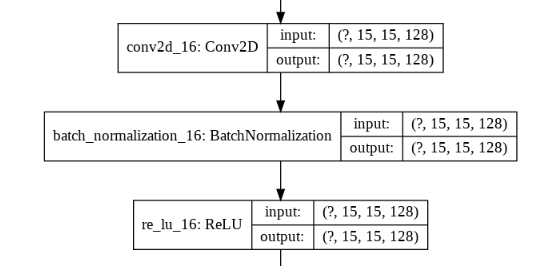
\includegraphics[width=0.4\textwidth]{img/vgg_layer.png}
            \caption{Capa VGG donde se puede ver la capa convolucional, la capa de batch normalization y la función de activación ReLU.}
            \label{fig:vgg_layer}
        \end{figure}
    
    \subsection{ResNet}
    
        \begin{figure}[t]
            \centering
            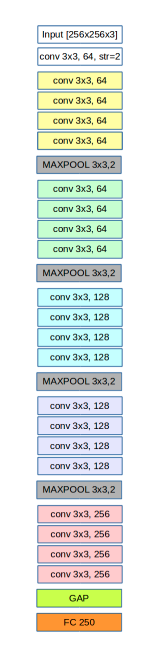
\includegraphics[width=0.15\textwidth]{img/vgg_arqr.png}
            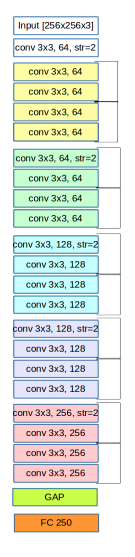
\includegraphics[width=0.15\textwidth]{img/resnet_arq.png}
            \caption{Arquitectura de las redes VGG y ResNet respectivamente. Obtenidas desde el enunciado de la tarea.}
            \label{fig:arqs}
        \end{figure}
        
        La arquitectura de ResNet se basa en el uso de la suma de los residuos de una red, es decir, tomar las características de una fase distinta de procesamiento (unas capas convolucionales atrás) y sumarla a la salida actual, para así poder seguir procesando. El propósito de esto es crear redes más profundas que las redes VGG comunes, llegando en (REFERENCIA AL PAPER DE RESNET) a ocho veces más capas convolucionales que la VGG. Con ello se planea conseguir un mayor nivel de accuracy que otras implementaciones anteriores.
        
        La arquitectura consiste en bloques de capas donde la salida de algunas capas es capturada más adelante en la red, donde la información es añadida y posteriormente procesada como una salida más. Esto se puede ver en la figura \ref{fig:resnet_block} donde la salida de una capa se divide en dos caminos, de los cuales uno es procesado por subsecuentes capas convolucionales, mientras que otro se mantiene intocable hasta el final, donde se añade a la salida procesada. Luego ambas salidas son procesadas por batchnormalization y la capa de activación ReLU.
        
        \begin{figure}[t]
            \centering
            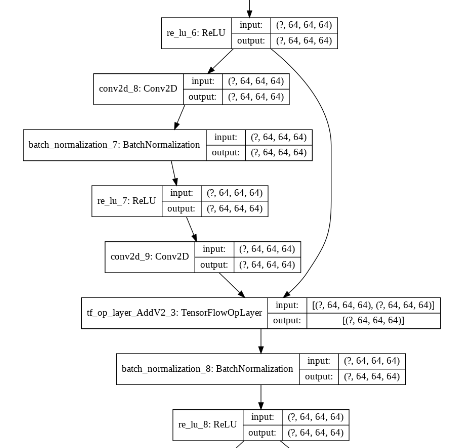
\includegraphics[width=0.4\textwidth]{img/resnet_layer.png}
            \caption{Bloque de capa resnet, donde la salida de capas anteriores va hacia adelante y es añadida a la salida de capas posteriores para agregar información de distinta escala semántica de características.}
            \label{fig:resnet_block}
        \end{figure}
        
        \begin{figure}[t]
            \centering
            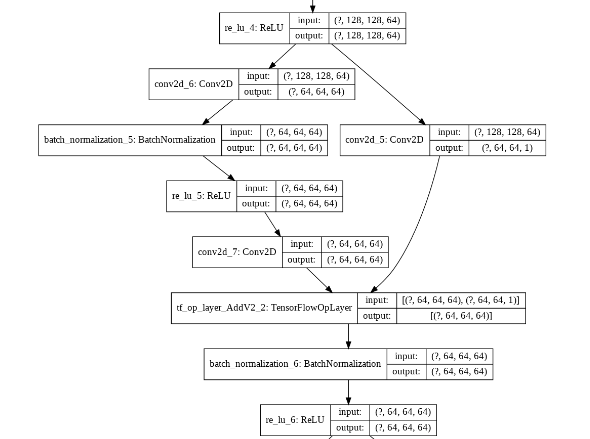
\includegraphics[width=0.48\textwidth]{img/resnet_layer2.png}
            \caption{Bloque resnet donde se debe tomar una reducción de la imagen para hacer calzar los tamaños del output de la rama interna con la externa.}
            \label{fig:resnet_block2}
        \end{figure}
        
        En una de las ramas que tiene el bloque de la resnet, se debe hacer una reducción de dimensionalidad como se puede apreciar la figura \ref{fig:resnet_block2}, la rama que no se pasa por las capas convolucionales se debe reducir ya que la primera capa convolucional de la rama, reduce la imagen a la mitad al aplicar un stride de 2.
        
        Debido a pruebas sobre los datos de entrenamiento, y para mejorar los resultados sobre el conjunto de test, se hace una prueba modificando la red, se añade una capa de \textit{dropout} en el GAP entre los bloques convolucionales y la última capa densa.
        
    \subsection{Squeeze \& Excitation}
    
        La red Squeeze \& Excitation consiste en la construcción de una rama paralela a las capas convolucionales de una red, donde se pueda dar un peso a cada uno de los canales de salida del bloque. Esto se realiza en (REFERENCIA AL PAPER) donde se argumenta que se realiza con el propósito de agregar información de relevancia a cada uno de los canales de una fase de convolución.
        
        \begin{figure}[t]
            \centering
            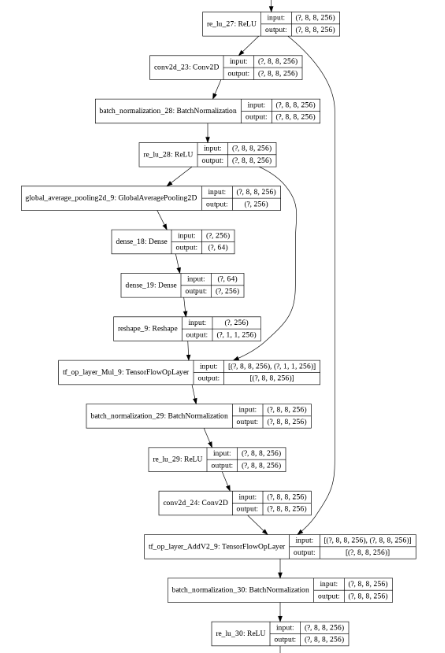
\includegraphics[width=0.48\textwidth]{img/squeeze_layer.png}
            \caption{Bloque de una red de Squeeze \& Excitation, donde se puede ver la rama del residuo en la derecha, mientras que en la parte izquierda se puede apreciar la implementación del paso de Squeeze y luego de Excitation.}
            \label{fig:squeeze_block}
        \end{figure}
        
        En la figura \ref{fig:squeeze_block} se puede apreciar la arquitectura básica de la red, donde el paso de \textit{Squeeze} se ve en la parte izquierda, donde la salida de las capas convolucionales anteriores se procesa con una capa de \textit{Global Averga Pooling}, la que consiste en comprimir todo el canal a un solo valor, como el promedio de los pixeles del \textit{feature map}. Luego, este arreglo de valores del largo de la cantidad de canales, es procesado por una capa densa con una salida reducida a un factor $C / r$ donde $C$ es la cantidad de canales y $r$ es un factor de reducción. Luego se amplifica la salida de esta capa con otra que iguala a los canales, posteriormente, estos valores se multiplican uno a uno con cada uno de los canales de salida de la capa convolucional que entra a la fase de \textit{Squeeze}, lo que se denomina \textit{Excitation}.
        
        Cabe mencionar que esta arquitectura se monta sobre la arquitectura de la resnet.

    \subsection{Implementación}

        La construcción de las redes fue hecha en \textbf{Colab} utilizando Keras, framework que permite la fácil implementación de las redes neuronales a través de tensores, donde una red se modela como un grafo y la interacción entre ellas como aristas en el grafo. Esta librería viene optimizada para el buen rendimiento y fácil manejo de las redes. La construcción se basa en la asignación de la salida de una capa convolucional a una \textit{variable} la cual se va procesando con capas de Keras. Luego se construye el modelo creando una instancia de \texttt{keras.models} la cual acepta como entrada este grafo conectado, y entrega una red neuronal que puede ser entrenada.
        
        Se utiliza \textbf{Colab} como plataforma para desarrollas, consiste en hardware disponible en la nube para correr modelos o procesos de alta exigencia computacional. Los datos con los que se entrena la red son bastante pesados (alrededor de 4GB cargados en memoria RAM como archivo numpy). En \textbf{Colab} se permite el uso de GPUs de alto rendimiento, con lo que el procesamiento de las imágenes y el entrenamiento en general se ve beneficiado por esto. Un entrenamiento que tarde semanas en una cpu, puede solo tardar horas o minutos en una o varias GPU.
        
        Luego de establecer estos criterios, se procede a construir las redes con Keras. Para ello se cargan las librerías predefinidas, se cargan los datos y luego se construye la red. La organización del código se puede ver en el mismo repositorio de la tarea, pero a grandes rasgos se siguen los siguientes pasos.
        
        \begin{enumerate}
            \item[1.] Carga de datos a arreglos \texttt{numpy}
                
            Los datos tienen un formato de punto flotante que toman un valor de 0 a 1.
            
            \item[2.] Se crea la instancia de las redes neuronales con \texttt{keras.models}
            
            Se utiliza \texttt{keras.layers} para construir la red, donde se implementan las convoluciones en dos dimensiones, las funciones de activación, max pooling, etc.
            
            \item[3.] Se entrena la red con \texttt{model.fit}
            
            Esta función tiene un comportamiento predefinido, donde se le entregan datos en una matriz de entrada con los datos ya cargados y transformados, también se le deben entregar las etiquetas de cada imagen. El problema de esta implementación es lo poco flexible en casos de querer hacer algo más complejo. Sin embargo, para el propósito de esta tarea se ocupa sin perjuicios, ya que la tarea llevada a cabo es de baja complejidad de implementación.
            
            \item[4.] El entrenamiento considera el uso de evaluaciones en tiempo real sobre el modelo, esto se realiza para obtener el mejor modelo sobre el conjunto de validación, en este caso el de test.
            
            Para monitorear esto, se crean funciones de callback, las cuales adquieren la salida del proceso de entrenamiento en línea, y realizan acciones como guardar \textit{checkpoints} del mejor modelo, o parar el funcionamiento de la red cuando llegue a cierto punto.
        \end{enumerate}
        
        Utilizando los pasos mencionados anteriormente se realiza el entrenamiento de cada una de las redes. Se obtiene el mejor modelo de cada una y posteriormente se comparan los resultados obtenidos sobre el conjunto de test.
        
        Cabe mencionar que se utiliza Colab junto con Drive (ambas son tecnologías de Google), la primera se utiliza para crear los modelos y visualizar los resultados, mientras que la segunda se utiliza para almacenar los modelos ya entrenados y almacenar el dataset que se utiliza para el entrenamiento y evaluación.

\section{Métricas de evaluación}
    
    Para evaluar el desempeño de los modelos se consideran 4 métricas de evaluación, las cuales se desglosan a continuación. Estas métricas son implementadas en Keras y en la librería sklearn, utilizada en el área de \textit{machine learning} con distintos modelos e implementaciones de investigaciones unos años atrás del estado del arte. En esta oportunidad se utilizan métricas de toda la vida.
    
    \subsection{\textit{Accuracy}}
    
        Esta métrica evalúa qué tan bien un modelo se desempeña en clasificar de forma correcta cierta cantidad de ejemplos. Se mide como
        
        \begin{equation}
            acc = \frac{\text{Correctas}}{\text{Total de ejemplos}}
        \end{equation}
        
        Por lo que esta métrica mide solamente la capacidad de discernir entre una etiqueta o la otra, sin importar si se equivoca sistemáticamente, etiqueta otros ejemplos con esta etiqueta o si la predicción se realiza con baja probabilidad.
    
    \subsection{\textit{Loss}}
        
        El \textit{loss} es una métrica de confianza que se tiene sobre el modelo, y de la seguridad que el modelo tiene al realizar las predicciones. Esto se debe a que considera la probabilidad de predicción considerada.
        
        \begin{equation}
            L = - \sum (y\log(p) + (1-y)\log(1-p))
        \label{eqn:log}
        \end{equation}
        
        En la ecuación \ref{eqn:log} se aprecia que la probabilidad es medida con el logaritmo, es decir, si se tiene baja probabilidad al contestar de forma correcta, de todas formas se presenta un alto valor de \textit{loss}. Mientras que si se equivoca con una confianza muy alta, también el valor de la \textit{loss} será muy alto.
        
        Esta función de pérdida es utilizada en el entrenamiento de las redes neuronales, ya que la probabilidad se puede modelar como una salida de la red que tenga una función \textit{Softmax} como salida. Y con ello se puede derivar la pérdida y optimizar los parámetros de la red.
        
        Es muy buena, ya que, como se menciona anteriormente, considera la etiqueta predicha y la confianza que se tiene en dicha predicción.
    
    \subsection{\textit{Recall}}
    
        Es una medida de relevancia durante la clasificación. Para medir el \textit{recall} se consideran los reales positivos predichos ($TP$) sobre el total de real positivos o la suma de los reales positivos predichos sobre los falsos negativos predichos ($FN$). Es una medida que da cuenta de la pregunta: \textit{Cuántos elementos reales positivos pude rescatar de todos los casos positivos}.
        
        El caso extremo de error al fijarse en solo esta métrica sería clasificar a todos los elementos como positivos, y tendría un \textit{recall} igual a 1, pero estaría erróneo el modelo.
    
    \subsection{\textit{F1-score}}
        
        Esta métrica resume en un solo valor la \textit{precision} ($p$) y el \textit{recall} ($r$) del modelo. \textit{Precision} se define como los casos reales positivos predichos sobre todos los positivos predichos (incluyendo a los falsos positivos). El \textit{f1-score} es una media armónica entre estas dos medidas.
        
        \begin{equation}
            F_1 = 2 \cdot \frac{p \cdot r}{p + r}
        \end{equation}
        
        Un valor igual a 1 de \textit{F1} sería obtener todos los positivos reales predichos con el modelo, sin ninguna equivocación sobre otras clases. Es decir, una distinción perfecta de la clase.
        
\section{Resultados Experimentales y Discusión}
    
    De la construcción e implementación de los modelos, se obtienen modelos con distinta cantidad de parámetros, los cuales son listados en la tabla \ref{tab:parametros}. Se puede notar que la cantidad de parámetros es similar en cada una de las arquitecturas, esto se debe a que la mayor fuente de parámetros son las capas convolucionales y las capas de \textit{batch normalization}, en este último caso, solo se añaden 4 parámetros por cada uno de los canales, es decir, si hay 64 salidas de una capa convolucional, tendremos 256 parámetros.
    
    Hay que recordar que las capas convolucionales añaden $(n_{in} \ \times \ 3 \ \times \  3 \ \times + 1) \ \times \ n_{out}$ parámetros en cada capa convolucional. Se considera que la primera capa solo tiene como input un solo canal, ya que las imágenes vienen en formato de un solo canal (con más canales se añade más peso computacional al programa).
    
    Cabe notar, que es coherente que en la tabla \ref{tab:parametros} la red con más parámetros sea la de Squeeze \& Excitation, ya que implementa capas densas en paralelo a las convolucionales.
    
    \begin{table}[t]
        \centering
        \begin{tabular}{c|cc}
             parametros & entrenables & no entrenables \\ \hline
            vgg & 3.537.914 & 5.248 \\
            resnet & 3.541.374 & 5.248 \\
            resnet + drop & 3.541.374 & 5.248 \\
            squeeze & 3.652.030 & 7.808 \\
        \end{tabular}
        \caption{Cantidad de parámetros por arquitectura}
        \label{tab:parametros}
    \end{table}
    
    Para analizar el rendimiento de las redes, se aplica una superposición de las curvas de \textit{loss} y \textit{accuracy} en la figura \ref{fig:train_plot} se observa como el entrenamiento se realiza por alguna cantidad de épocas inferior a 20. Número que es considerado pequeño para modelos reales, los cuales tienen una convergencia más lenta pero con mejores resultados a la larga.
    
    En este caso, se aplica \textit{early stopping} para obtener el mejor modelo, se aplica una paciencia de 4 épocas, por lo que el entrenamiento al encontrar el modelo de menor \textit{loss} espera 4 épocas para parar, a menos que encuentre un nuevo modelo con mejor rendimiento.
    
    \begin{figure}[t]
        \centering
        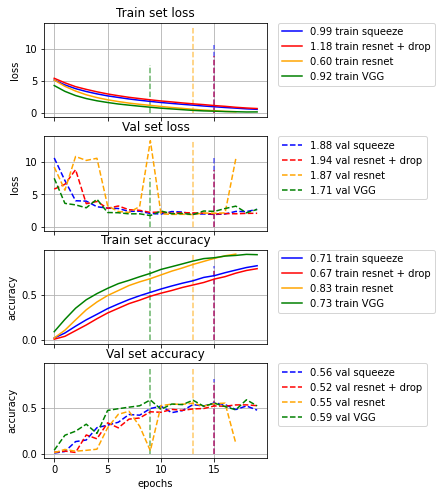
\includegraphics[width=0.48\textwidth]{img/train_plot.png}
        \caption{Fase de entrenamiento de las redes neuronales. Se puede ver como los modelos progresan en el \textit{accuracy} mientras minimizan el \textit{loss}. Se grafica con una línea vertical el punto de menor \textit{loss} sobre el conjunto de test, donde se continúa el entrenamiento por algunas épocas más en el caso de que mejore en la \textit{loss}.}
        \label{fig:train_plot}
    \end{figure}
    
    Se puede observar de la figura \ref{fig:train_plot} que la red VGG es la que tiene una convergencia más rápida a un mínimo en la \textit{loss}. También se ve que las rede más complejas tienen una convergencia más lenta. En particular, durante la experimentación se observó que el agregar \textit{dropout} a la resnet se aumenta el tiempo de convergencia, comparada con la ResNet sin dicha regularización.
    
    Los resultados mostrados anteriormente, dan cuenta de que los modelos tienen un comportamiento similar en el conjunto de test, donde los resultados son bastante similares y poco concluyentes en el sentido de mejora con alguna de las arquitecturas propuestas. De hecho, lo que uno esperaría es lo contrario a lo que sucede en la fase de entrenamiento, ya que el modelo más simple es el que tiene mejor rendimiento.
    
    Una conjetura de a qué se debe esto, es que la arquitectura sugerida, por ejemplo en ResNet, no considera que se agreguen más bloques de convolución, sino que la cantidad agregada es similar a la de la VGG, por lo que el principio que inspira la arquitectura, se perdería.
    
    Cabe destacar un fenómeno que ocurre en el \textit{accuracy} sobre el test durante el entrenamiento. Este valor aumenta constantemente a medida que se entrena, independiente del \textit{loss} hasta cierto punto. Esto se debe a que el \textit{accuracy} y \textit{loss} miden cosas diferentes. El primero mide qué tan bien el modelo logra apuntarle a la etiqueta correcta, mientras no se preocupa de la cantidad de veces que este se equivoca. Por otro lado, el \textit{loss} penaliza cada vez que se equivoca, y este valor dependerá de la magnitud de dicha equivocación.
    
    En la ecuación \ref{eqn:log} se aprecia la función de \textit{loss}, en esta se puede ver que su valor dependerá también de la probabilidad con la que el modelo prediga un respectivo label. Con lo que si de todas formas le apunta correctamente a cada una de las etiquetas, aún puede presentar una \textit{loss} positiva, hasta que la probabilidad predicha sea igual a 1.
    
    \begin{table}[t]
        \centering
        \begin{tabular}{c|ccc}
             & $acc$ & recall & F1-score\\ \hline
            VGG & 0.63 & 0.59 & 0.59 \\
            RN & 0.57 & 0.52 & 0.51 \\
            RN + Dropout & 0.57 & 0.52 & 0.51 \\
            SE & 0.61 & 0.56 & 0.55 \\
        \end{tabular}
        \caption{\textit{Accuracy}, \textit{recall} y \textit{F1-score} promedio sobre las clases obtenidos por cada uno de los modelos.}
        \label{tab:metrics}
    \end{table}
    
    Como se mencionaba anteriormente, el de mejor rendimiento se ve reflejado en la tabla \ref{tab:metrics}, donde VGG se lleva el mejor rendimiento en todas las métricas utilizadas.
    
    \subsection{Algunas visualizaciones}
    
        A continuación, se analizan los resultados obtenidos por clase, donde se evalúa según el \textit{accuracy}, \textit{recall} y \textit{F1-score} individual de cada clase. Se parte con las clases que obtuvieron mejores resultados de forma general, es decir, a lo largo de los cuatro modelos.

\subsection{Conclusiones}
    
    Con este trabajo se logró familizarizarse con el framework de trabajo para la creación de redes neuronales y así contribuir a la formación como profesional, ya que las redes neuronales cada vez cobran mayor terreno en aplicacaiones de toda índole.
    
    Además, de la construcción de redes neuronales, se exponen resultados adecuados en el entrenamiento de las mismas redes y se realiza un análisis de por qué se obtienen dichos resultados. Cabe destacar que no se obtienen los esperados por los trabajos en los que se basa la presente tarea, sin embargo, se tiene bajo consideración que por lo mismo es solamente una tarea.
    
    Dentro de la evaluación de las distintas arquitecturas, se ve un comportamiento del cual se tenía desconocimiento, y es la diferencia entre el \textit{accuracy} y el \textit{loss}, ya que siempre se creía erróneamente que el \textit{accuracy} es el indicador más importante, sin embargo, puede llevar a malas interpretaciones y elecciones erróneas de modelo, es por ello que se entrena mirando el \textit{loss} en el caso de la elección del mejor modelo.
    
    Como trabajo a futuro, se podría investigar en la implementación de una ResNet más grande sobre el mismo set de datos, para acercarse a resultados del estado del arte.
    
% \begin{thebibliography}{}

% \bibitem[He2016] He, Kaiming and Zhang, Xiangyu and Ren, Shaoqing and Sun, Jian, \emph{Deep residual learning for image recognition}, Proceedings of the IEEE Computer Society Conference on Computer Vision and Pattern Recognition, 2016

% \end{thebibliography}